% This file is iccc.tex.  It contains the formatting instructions for and acts as a template for submissions to ICCC.  It borrows liberally from the AAAI and IJCAI formats and instructions.  It uses the files iccc.sty, iccc.bst and iccc.bib, the first two of which also borrow liberally from the same sources.


\documentclass[letterpaper]{article}
\usepackage{iccc}

\usepackage{graphicx}       % figures
\usepackage{float}

\usepackage{times}
\usepackage{helvet}
\usepackage{courier}
\pdfinfo{
/Title (SpaceSheet: Navigating Conceptual Space with a Spreadsheet Interface)
/Subject (Proceedings of ICCC)
/Author (ICCC)}
% The file iccc.sty is the style file for ICCC proceedings.
%
\title{SpaceSheet: Navigating Conceptual Space with a Spreadsheet Interface}
\author{
  Anonymous Author(s)\\
  Anonymous School(s)\\
  \texttt{\{Anonymous Email(s)\}} \\
}
\setcounter{secnumdepth}{0}

\begin{document} 
\maketitle
\begin{abstract}
\begin{quote}
We introduce a new spreadsheet based interface call SpaceSheets for creating novel images and other media. Unlike traditional digital tools, ours is parameterized entirely by a neural network with no preprogrammed rules or knowledge representations. The capability of SpaceSheets to support visual exploration and communication is demonstrated within the context of several domains including facial images, fonts, and english words. SpaceSheets is demonstrated to support the experimentation and exploration of latent spaces enabling more effective design experimentation.
\end{quote}
\end{abstract}

\section{Introduction}

Problem solving can be viewed as a search for a solution within a space. In design, this process involves generating solutions and evaluating their consequences relative to goals and constraints~\cite{simon95}. These experiments are enabled through representations in the form of drawings and diagrams. Computational design tools enable users to construct and manipulate representations digitally. These tools often impose a high cost to design experimentation due to the mismatch between low-level design operations in expressing more abstract design intent.

Generative models learn more compact representations of the training data in a vector space of latent variables. Latent variables are sampled from high-dimensional latent space and can be decoded back into observable values. Additionally, semantic operations can be performed within latent space using vector arithmetic~\cite{white16}.

Spreadsheet interfaces are a ubiquitous part of office productivity suites. They enable users to perform experimental calculations using a set of formulae which define relationships spatially. Automatic recalculation supports experimentation by enabling users to observe the results of their actions immediately and act accordingly

\begin{figure}[ht]
  \centering
  % \fbox{\rule[-.5cm]{0cm}{4cm} \rule[-.5cm]{4cm}{0cm}}
  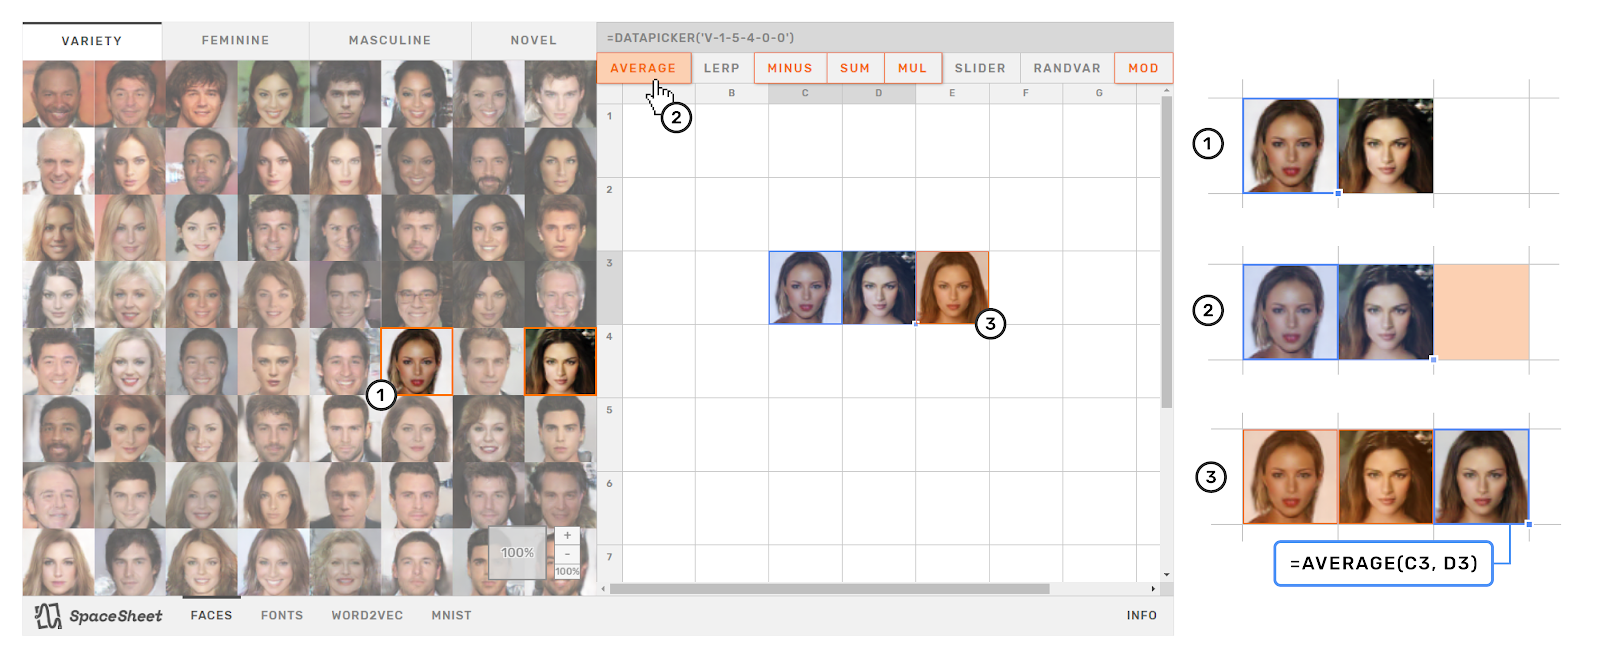
\includegraphics[width=8cm]{figs/01-hero-diagram.png}
  \caption{The SpaceSheet being used to perform an average between two latent variables}
\end{figure}

We developed SpaceSheet (Figure 1) to leverage the familiarity and power of spreadsheet interfaces for the purpose of design experimentation within latent space. It has been adapted to enable non- experts to explore and experiment within latent spaces.

\section{Background}

\subsection{Conceptual Spaces}

Generative models are a popular approach to unsupervised machine learning. Generative neural network models are trained to produce data samples that resemble the training set ~\cite{openai1}. Because the number of model parameters is significantly smaller than the training data, the models are forced to discover efficient data representations. These models are sampled from a set of latent variables in a high dimensional space, called a latent space. Latent space can be sampled to generate observable data values. Learned latent representations often also allow semantic operations with vector space arithmetic (Figure 2), a phenomenon discovered previously in the latent space of language models~\cite{wordvec}.

\begin{figure}[ht]
  \centering
  % \fbox{\rule[-.5cm]{0cm}{4cm} \rule[-.5cm]{4cm}{0cm}}
  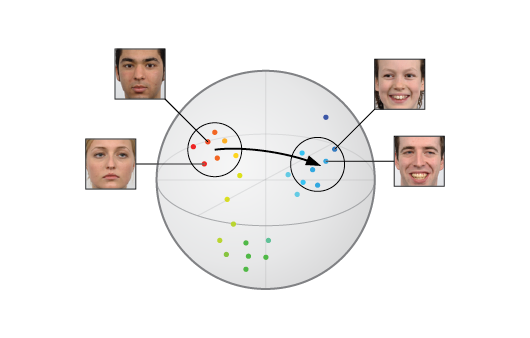
\includegraphics[width=8cm]{figs/face_space.png}
  \caption{Schematic of the latent space of a generative model. In the general case, a generative model includes an encoder to map from the feature space (here images of faces) into a high dimensional latent space. Vector space arithmetic can be used in the latent space to perform semantic operations. The model also includes a decoder to map from the latent space back into the feature space, where the semantic operations can be observed. If the latent space transformation is the identity function we refer to the encoding and decoding as a reconstruction of the input through the model. }
\end{figure}


\bibliographystyle{iccc}
\bibliography{iccc,spacesheet}


\end{document}
